\documentclass[11pt]{article}

% ============================================================
%  ARC Disaster-Response Game --- Mechanics Formalization
%  Scope: Unity game mechanics + the gym (env) interface boundary.
%  Style: descriptive specification of intended/effective mechanics.
%         The Python reward/scoring layer is deferred to a companion doc.
% ============================================================

\usepackage[margin=1in]{geometry}
\usepackage{amsmath,amssymb}
\usepackage{booktabs}
\usepackage{longtable}
\usepackage{enumitem}
\usepackage{xcolor}
\usepackage{algorithm}
\usepackage{algpseudocode}
\usepackage{tikz}
\usetikzlibrary{automata,positioning,arrows.meta}
\usepackage{hyperref}
\hypersetup{colorlinks=true,linkcolor=blue!50!black,urlcolor=blue!50!black}

\newcommand{\code}[1]{\texttt{\small #1}}
\newcommand{\file}[1]{\textcolor{blue!40!black}{\texttt{\footnotesize #1}}}
\newcommand{\Round}{r}
\newcommand{\Day}{d}
\newcommand{\seg}{s}

\title{\textbf{The ARC Disaster-Response Game}\\[2pt]
\large A Formal Specification of Game Mechanics\\[4pt]
\normalsize (Unity engine + gym interface boundary)}
\author{CORA / ARC\_Game}
\date{\today}

\begin{document}
\maketitle

\begin{abstract}
This document formalizes the mechanics of the ARC disaster-response management
game as implemented in the Unity engine and exposed to decision-making policies
(LLMs and non-learning heuristics) through the TCP gym interface. It defines the
temporal model, the action space and its enumeration, the task lifecycle,
building and worker mechanics, client--stay and casework dynamics, transportation
and delivery, the flooding/weather stochastic layer, and the budget/termination
economy. All numeric constants reflect the \emph{headless gym build}, which is
the configuration policies actually run against; where a value is decided in the
Python action layer rather than in Unity, this is stated explicitly. The
Python-side reward function is intentionally out of scope and treated as a
separate artifact; here we document only the raw quantities Unity reports.
\end{abstract}

\tableofcontents
\bigskip

% ============================================================
\section{Overview and Notation}
% ============================================================

The player (``Director'') manages a disaster-relief operation over a fixed
horizon. Each round the player may build and deconstruct facilities, hire and
train workers, assign workers to facilities, transfer resources, and respond to
\emph{tasks} (events) by selecting among offered choices. Decisions consume a
shared \emph{budget} and influence \emph{satisfaction}; floods and weather
perturb the map and block delivery routes. The objective (scored externally in
Python) rewards meeting population needs (food, lodging, casework/return-home)
while spending efficiently.

\paragraph{Agent--environment loop.}
A policy interacts with the game through the gym wrapper
(\file{arc\_game\_gym\_env\_tcp.py}) over TCP to a headless Unity process
(\file{GymServerManager.cs}). Each environment \emph{step} consists of (i)
executing zero or more queued actions, then (ii) advancing the simulation by
exactly one round, then (iii) returning the updated game state. The detailed
ordering is given in \S\ref{sec:temporal}.

\paragraph{Notation.} Table~\ref{tab:notation} lists recurring symbols.

\begin{table}[h]
\centering
\small
\begin{tabular}{@{}ll@{}}
\toprule
Symbol & Meaning \\
\midrule
$\Day \in \{1,\dots,8\}$ & current day \\
$\seg \in \{0,1,2,3\}$ & time segment within a day ($9{:}00,12{:}00,15{:}00,18{:}00$) \\
$\Round = 4(\Day-1)+\seg+1$ & global round index ($1$--$32$); $0$-based in the payload \\
$B$ & current budget (dollars) \\
$\Sigma$ & current satisfaction, $\Sigma \in [0,100]$ \\
$W_T, W_U$ & free trained / untrained worker counts \\
$\omega(\cdot)$ & workforce value: $\omega(\text{trained})=2,\ \omega(\text{untrained})=1$ \\
$\rho_b$ & required workforce of building $b$ (always $4$ for constructables) \\
$\mathrm{cap}_b^{\text{pop}}, \mathrm{cap}_b^{\text{food}}$ & population / food capacity of building $b$ \\
$n_b$ & current occupancy (population) of building $b$ \\
\bottomrule
\end{tabular}
\caption{Notation.}
\label{tab:notation}
\end{table}

\paragraph{Source-of-truth convention.} Numeric constants are defined
canonically in the Unity build; we annotate these \textbf{(U)}. The gym action
layer transmits a per-action \code{cost} that Unity charges verbatim, so the
charge mechanism lives in Python while the \emph{value} must mirror the Unity
canonical constant --- the two are required to stay in sync. A few quantities
exist \emph{only} in the Python action layer (the resource-transfer quantity
menus and the per-action hire-bundle cap); these are annotated \textbf{(P)}.
Quantities overridable by external config are annotated \textbf{(cfg)}.

% ============================================================
\section{Temporal Model and the Step Sequence}
\label{sec:temporal}
% ============================================================

\subsection{Discrete time}
Time is partitioned into \emph{days} and \emph{rounds}. There are $4$ rounds
(time segments) per day and at most $8$ days, giving a maximum horizon of
\[
  \Round_{\max} = 4 \times 8 = 32 \text{ rounds.}
\]
The natural episode terminus is the end of Day~8, Round~4
(\file{GlobalClock.cs}), and the benchmark harness plays the full $32$-round
horizon. The gym wrapper exposes a \code{max\_episode\_steps} cap (one step $=$
one round) as a safety bound; it is set at or above $32$ so it does not truncate
a normal episode --- the episode ends at the natural Day~8/Round~4 terminus (or
early on satisfaction collapse, \S\ref{sec:economy}). Round indexing in
the serialized payload is $0$-based ($\Round\!-\!1$).

\subsection{One round of wall-clock simulation}
In headless mode a round is advanced by a single \code{advance\_time} request,
which runs one \emph{simulation coroutine}. The coroutine spins for a fixed
game-time budget using a fixed capture timestep:
\[
  \Delta t = 0.3\ \text{game-s/frame}, \qquad
  T_{\text{round}} = 10\ \text{game-s}, \qquad
  N_{\text{frames}} = \lceil T_{\text{round}}/\Delta t \rceil = 34 .
\]
Thus roughly $10.2$ game-seconds elapse per round. This matters because several
in-engine timers are expressed in game-seconds (construction $5$\,s,
deconstruction $3$\,s); since each is shorter than one round's budget, they
\emph{complete within the same round} in which they start
(\S\ref{sec:buildings}).

\subsection{Ordering within a step}
The precise order of effects in a single environment step is given in
Algorithm~\ref{alg:step}. The key consequence for policies: \textbf{queued
actions are applied before the simulation runs}, and \textbf{within-round
resolutions (deliveries arriving, tasks expiring, food produced/consumed, costs
billed) become observable only in the state returned at the end of the step.}

\begin{algorithm}[h]
\caption{Environment step (one round)}
\label{alg:step}
\begin{algorithmic}[1]
\State \textbf{Input:} list of action indices $A$ (possibly empty), choice selections
\For{each action $a \in A$} \Comment{all execute \emph{before} time advances}
  \State \Call{ExecuteAction}{$a$} \Comment{build/deconstruct, hire/train/assign, queue transfer}
  \State deduct $\mathrm{cost}(a)$ from $B$; mutate worker pools / sites immediately
\EndFor
\For{each pending choice selection} \Comment{\code{select\_task\_choice}}
  \State apply choice impacts (satisfaction now; budget now if cost, scheduled if income)
  \State trigger immediate delivery, or enqueue a vehicle delivery (\S\ref{sec:transport})
\EndFor
\If{$\seg \geq 4$} \Comment{day boundary reached on the previous round}
  \State \Call{ProceedToNextDay}{} : $\Day \mathbin{+}{=}1$; $\seg \gets 0$
  \State fire \textsc{OnDayChanged}: charge motel occupancy cost; clear food waste
\EndIf
\State \Call{RunSimulationCoroutine}{$T_{\text{round}}$} \Comment{$\sim$10\,s of physics}
  \Statex \hspace{1.5em} vehicles move/deliver; construction \& deconstruction coroutines finish;
  \Statex \hspace{1.5em} kitchens produce food; shelters/community consume food; task timers tick
\State \Call{EndSimulation}{} :
  \Statex \hspace{1.5em} \textsc{RewardMetricsTracker.OnRoundEnded} (snapshot worker person-rounds)
  \Statex \hspace{1.5em} $\seg \mathbin{+}{=}1$; fire \textsc{OnRoundEnd} (apply matured delayed-budget items)
  \Statex \hspace{1.5em} check end-of-day / end-of-game
\State \Return serialized \code{GameStatePayload}; re-enumerate valid actions
\end{algorithmic}
\end{algorithm}

\subsection{Initial state (reset)}
A fresh episode initializes to: $\Day=1,\ \seg=0$; budget $B=10000$ and
satisfaction $\Sigma=50$ (both overridable by config, \S\ref{sec:economy});
worker pool of $5$ trained $+\ 5$ untrained, all immediately free; the prebuilt
map (Community at full occupancy, Motel empty, abandoned construction sites);
and no player-built facilities. Tasks are generated on demand each round
(\S\ref{sec:tasks}).

% ============================================================
\section{Action Space}
\label{sec:actions}
% ============================================================

\subsection{Enumeration and the round trip}
Before each decision the action layer (\file{action\_enumerator.py}) enumerates
\emph{all currently valid actions} from the latest game state, producing an
indexed list. A policy selects one or more indices; the gym serializes each
selected action to JSON and sends it to Unity, where \code{ActionExecutor}
deserializes it into a \code{GameAction} and applies the corresponding effect,
charging exactly the \code{cost} field carried in the message. After the round
advances, the action list is regenerated, so \emph{indices are not stable across
rounds}.

There are six action families. Five are enumerated mutating actions; the sixth,
\code{select\_task\_choice}, answers a task (\S\ref{sec:tasks}) and is issued
through a dedicated path rather than the mutating-action list.

\begin{table}[h]
\centering\small
\begin{tabular}{@{}lll@{}}
\toprule
Family & Cost & Availability predicate (enumeration gate) \\
\midrule
\code{construction}       & \$1000 & site available $\wedge\ B \geq 1000$ \\
\code{worker} (hire/train) & see \S\ref{sec:actions:worker} & budget/pool gates (no daily cap) \\
\code{worker\_assignment} & \$0 & building $\in\{$NeedWorker, InUse$\}\ \wedge$ unmet workforce \\
\code{resource\_transfer} & \$0 & a vehicle available $\wedge$ source stock $\wedge$ dest space \\
\code{deconstruction}     & \$0 & target is a player-built building \\
\code{select\_task\_choice} & impacts of the choice & task active $\wedge$ choice feasible \\
\bottomrule
\end{tabular}
\caption{Action families.}
\label{tab:actions}
\end{table}

\subsection{Construction}
For each available abandoned site and each constructable type
$\tau \in \{\text{Kitchen},\text{Shelter},\text{CaseworkSite}\}$ with
$B \geq 1000$, one action \code{build\_$\tau$\_\{site\}} is enumerated. Executing
it deducts \$1000, marks the site occupied, and creates the building in status
\textsc{UnderConstruction}. The building completes (transitions to
\textsc{NeedWorker}) within the same round (\S\ref{sec:temporal}).

\subsection{Workers: hire and train}
\label{sec:actions:worker}
Worker actions are \emph{quantity-bundled}: for an affordable quantity range the
enumerator emits one action per quantity $q$, with cost linear in $q$. There is
\textbf{no per-day hiring ceiling} --- hiring is bounded only by the budget. A
per-action bundle cap $M_{\text{hire}} = 5$ (and $M_{\text{train}}=10$)
\textbf{(P)} keeps the enumerated list bounded; a policy may still hire every
round and issue multiple hire actions per step, so cumulative hiring is
unlimited.

\begin{align}
\text{hire untrained:} &\quad \mathrm{cost} = 100\,q, &
  q &\in \{1,\dots,\min(\lfloor B/100\rfloor,\ M_{\text{hire}})\} \\
\text{hire trained:} &\quad \mathrm{cost} = 300\,q, &
  q &\in \{1,\dots,\min(\lfloor B/300\rfloor,\ M_{\text{hire}})\} \\
\text{train untrained:} &\quad \mathrm{cost} = 500\,q, &
  q &\in \{1,\dots,\min(W_U,\ \lfloor B/500\rfloor,\ M_{\text{train}})\}
\end{align}

In the headless build, hiring and training are \emph{instantaneous}: a hired or
newly trained worker is immediately available (status \textsc{Free}); there is
no arrival delay and no multi-round training period. Training converts one
untrained worker ($\omega=1$) into one trained worker ($\omega=2$) in place.
Note the resulting economics: training a worker (\$500) costs \emph{more} than
hiring a trained worker outright (\$300), so under these constants direct
trained-hire dominates training as a way to add trained
workforce.\footnote{The interactive (human) build routes hiring/training through
separate request/training systems with arrival delays; those paths are not
exercised by the gym and are out of scope here. The worker costs above are the
canonical Unity values (\$100/\$300/\$500), which the gym action layer mirrors
and charges.}

\subsection{Worker assignment}
For each building needing workforce, the enumerator emits assign actions in both
worker classes for quantities up to the shortfall. Let the shortfall be
$\delta_b = \rho_b - \text{assigned}(b)$. The executor assigns
\emph{trained-first, then untrained} to satisfy the requested headcount, drawing
from the free pools, and updates building status when
$\sum \omega(\cdot) \geq \rho_b$ (\S\ref{sec:workers}).

\subsection{Resource transfer}
For each ordered (source, destination) facility pair and each fixed quantity in a
preset menu, a transfer is enumerated when source stock and destination free
space both admit it and a vehicle is available:
\[
\text{food packs: } q \in \{10,25,50,100\}, \qquad
\text{population: } q \in \{5,10,20\}.
\]
The transfer costs nothing to issue; it creates a vehicle delivery task that
resolves over the round (\S\ref{sec:transport}).

\subsection{Deconstruction}
For each player-built building, \code{deconstruct\_\{name\}} is enumerated.
Executing it releases all assigned workers back to the free pool and begins
deconstruction, which completes within the same round, freeing the site for
future construction.

% ============================================================
\section{Tasks}
\label{sec:tasks}
% ============================================================

\subsection{Data model}
A \code{GameTask} bundles: a type and optional tag, an affected facility, a
countdown \code{roundsRemaining}, a list of \emph{impacts}
(signed deltas on Satisfaction, Budget, FoodPacks, Clients, Workforce, \dots),
and a list of \emph{choices} (\code{AgentChoice}). Population/lodging tasks also
carry a \code{demandQuantity} (people needing service) and an accumulating
\code{deliveredQuantity}. A choice carries its own impacts and an optional
\emph{delivery configuration} (\S\ref{sec:transport}).

\subsection{Types and tags}
The \emph{type} sets the response window and penalty semantics; the \emph{tag}
routes the task into reward accounting.

\begin{table}[h]
\centering\small
\begin{tabular}{@{}lll@{}}
\toprule
Type & Default window & Expiry semantics \\
\midrule
Emergency & 1 round & on expiry: incomplete; impacts (penalties) applied \\
Demand    & 2 rounds & on expiry: incomplete; impacts (penalties) applied \\
Advisory  & 3 rounds & may be ignored with no penalty \\
Alert     & 2 rounds & handled globally; not an interactive task-center item \\
Other     & --- & non-displaying; auto-dismissed \\
\bottomrule
\end{tabular}
\quad
\begin{tabular}{@{}ll@{}}
\toprule
Tag & Reward routing \\
\midrule
Food & food resolved/fulfilled \\
Lodging & lodging resolved/fulfilled \\
BackToHome & casework/return-home \\
None & not scored \\
\bottomrule
\end{tabular}
\caption{Task types (left) and tags (right).}
\label{tab:tasktypes}
\end{table}

\subsection{Generation}
At the start of each round the task system evaluates a database of task
templates. Each template is gated by one or more \emph{triggers} combined with
AND or OR logic, evaluated per eligible facility (or once globally for global
tasks). Duplicate suppression prevents re-spawning an identical
(facility, title) task that is already active. The trigger taxonomy:

\begin{itemize}[nosep]
\item \textbf{Deterministic:} Round, Day (specific/interval/range/from),
  Resource threshold (empty/full/$<$/$>$), Budget, Satisfaction, Workforce,
  FacilityStatus, Weather, FloodTile count, FloodedFacility (proximity).
\item \textbf{Stochastic:} Probability trigger --- fires when a fresh uniform
  draw $u \sim U[0,1)$ satisfies $u < p$, evaluated independently per facility.
  Community-request generation similarly uses a per-community Bernoulli$(0.5)$.
\end{itemize}

Flood-driven tasks (road blockage, vehicle repair) are event-driven, emitted
when the flood layer expands onto a route or a vehicle is caught
(\S\ref{sec:flood}). Because probability triggers, weather, and floods draw from
an unseeded RNG, task generation is \emph{stochastic across episodes}
(\S\ref{sec:flood:rng}).

\subsection{Choice feasibility (gating)}
A choice with no delivery is always feasible. A delivery choice is feasibility-
checked before being offered as selectable:
\begin{itemize}[nosep]
\item \textbf{Food delivery:} immediate (airlift) variants are always feasible;
  deferred variants require kitchen stock and an available vehicle.
\item \textbf{Population relocation:} requires destination capacity --- shelter
  space if routing to shelters, motel space if routing to motels.
\item \textbf{Return-home / casework:} routing to a CaseworkSite is treated as
  processing-home and is \emph{not} gated on shelter/motel space, so the
  casework option is never hidden when it is the intended response.
\end{itemize}
An infeasible choice is shown with a reason but cannot be selected.

\subsection{Resolution and fulfillment accounting}
Selecting a choice applies its impacts immediately (satisfaction; budget cost
immediately, budget income possibly delayed --- \S\ref{sec:economy}) and either
completes the task at once (no delivery), or sets it \textsc{InProgress} pending
delivery completion. A task ends as \textsc{Completed} (fully serviced),
\textsc{Incomplete} (expired with penalties), or ignored (Advisory).

For Food/Lodging-tagged tasks the metrics tracker records, at resolution,
\[
  \text{resolved} \mathbin{+}{=} \begin{cases} D & D>0\\ 1 & D=0\end{cases},
  \qquad
  \text{fulfilled} \mathbin{+}{=} \begin{cases} \min(\text{delivered}, D) & D>0\\
     \mathbb{1}[\text{serviced}] & D=0,\end{cases}
\]
where $D=\code{demandQuantity}$. For a Lodging task, $D$ is set at creation to
the \emph{maximum} delivery quantity across the task's choices. A delivery that
arrives \emph{after} the task has closed (a ``late delivery'') still increments
the fulfilled count (capped at resolved), crediting service that physically
occurred.

% ============================================================
\section{Buildings and Capacities}
\label{sec:buildings}
% ============================================================

\subsection{Inventory of building types}
Table~\ref{tab:buildings} lists every building. Constructable buildings cost
\$1000, require workforce $4$, and are built on abandoned sites; prebuilt
buildings exist from the start and need no workforce.

\begin{table}[h]
\centering\small
\begin{tabular}{@{}lcccccl@{}}
\toprule
Building & Kind & Pop cap & Food cap & Workforce & Cost & Role \\
\midrule
Kitchen      & constructable & --- & 20 & 4 & \$1000 & produces 10 food/round \\
Shelter      & constructable & 10 & 10 & 4 & \$1000 & houses people; consumes food \\
CaseworkSite & constructable & 40 & --- & 4 & \$1000 & processes people home \\
Community    & prebuilt & 40 & 40 & --- & --- & origin population (starts full); consumes food \\
Motel        & prebuilt & 300 & --- & --- & --- & overflow lodging; \$200/person/day \\
\bottomrule
\end{tabular}
\caption{Building inventory and capacities (headless build).}
\label{tab:buildings}
\end{table}

\subsection{Status automaton}
Every building moves through a status lifecycle (Fig.~\ref{fig:status}). A
constructable starts \textsc{UnderConstruction}; on completion it becomes
\textsc{NeedWorker}; once enough workforce is assigned
($\sum\omega \geq \rho_b = 4$) it becomes \textsc{InUse} and is
\emph{operational} (only operational buildings produce/consume and can
source/receive deliveries). Losing workforce drops it back to
\textsc{NeedWorker}. Deconstruction releases workers and removes the building.

\begin{figure}[h]
\centering
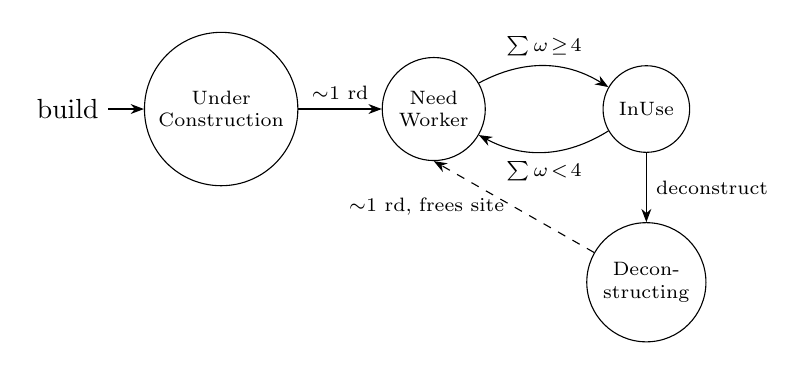
\begin{tikzpicture}[->,>=Stealth,node distance=2.7cm,on grid,auto,
  every state/.style={draw,minimum size=1.1cm,font=\scriptsize,align=center}]
  \node[state,initial,initial text=build] (uc) {Under\\Construction};
  \node[state,right=of uc] (nw) {Need\\Worker};
  \node[state,right=of nw] (iu) {InUse};
  \node[state,below=2.2cm of iu] (dc) {Decon-\\structing};
  \path
    (uc) edge node[above,font=\scriptsize]{$\sim$1 rd} (nw)
    (nw) edge[bend left] node[above,font=\scriptsize]{$\sum\omega\!\geq\!4$} (iu)
    (iu) edge[bend left] node[below,font=\scriptsize]{$\sum\omega\!<\!4$} (nw)
    (iu) edge node[right,font=\scriptsize]{deconstruct} (dc)
    (dc) edge[dashed] node[left,font=\scriptsize]{$\sim$1 rd, frees site} (nw.south);
\end{tikzpicture}
\caption{Building status lifecycle. Construction and deconstruction timers
($5$\,s and $3$\,s of game time) each complete within a single round.}
\label{fig:status}
\end{figure}

\subsection{Food production and consumption}
A Kitchen, when operational, produces a fixed amount per round up to its food
capacity:
\[
  \text{food}_{\text{Kitchen}}(\Round{+}1) =
  \min\!\big(\mathrm{cap}^{\text{food}}_{\text{Kitchen}},\
  \text{food}_{\text{Kitchen}}(\Round) + 10\big).
\]
Buildings with population-based consumption enabled (Shelter, Community) consume
one food pack per resident per $\kappa = 4$ rounds. Letting $c_b(\Round)$ be a
per-building consumption phase counter,
\[
  c_b \mathbin{+}{=} 1; \quad \text{if } c_b \equiv 0 \ (\mathrm{mod}\ \kappa):\quad
  \text{food}_b \mathbin{-}{=} n_b
  \quad(\text{capped at available stock}).
\]
Motel and CaseworkSite do not consume food. Unconsumed food may be cleared at the
day boundary (food-waste rule). Workers do not consume food in the current
configuration.

% ============================================================
\section{Workers}
\label{sec:workers}
% ============================================================

\subsection{Pools and workforce value}
Workers are \emph{trained} ($\omega=2$) or \emph{untrained} ($\omega=1$) and
occupy one of the statuses \textsc{Free}, \textsc{Working}, or (untrained only)
\textsc{Training}. The available workforce is
\[
  \Omega_{\text{free}} = 2\,W_T + W_U .
\]
The episode begins with $5$ trained and $5$ untrained workers
($\Omega = 2\cdot5 + 5 = 15$), all free.

\subsection{Assignment}
\code{TryAssignWorkersToBuilding}$(b, q)$ fills building $b$ toward its required
headcount by drawing \emph{trained workers first, then untrained}, setting each
chosen worker to \textsc{Working} bound to $b$, until either $q$ workers are
placed or the free pools are exhausted. A building activates
(\textsc{NeedWorker} $\to$ \textsc{InUse}) once its assigned workforce value
reaches $\rho_b = 4$; e.g.\ two trained workers ($2\times2$) or four untrained
($4\times1$) suffice.

\subsection{Person-round accounting}
At each round end the metrics tracker accumulates worker allocation as
person-rounds, $\sum_\Round(\text{working}, \text{training}, \text{idle})$,
forming the basis for the externally computed labor-cost/utilization terms.
These are reported raw; no scoring is applied in Unity.

% ============================================================
\section{Client Stay and Casework}
\label{sec:casework}
% ============================================================

People relocated into lodging (Shelter or Motel) are tracked as \emph{client
groups} with an arrival round. The relevant round measure is
$\Round = 4(\Day-1) + \seg$. A group's residence duration drives the
return-home (casework) dynamics:

\begin{itemize}[nosep]
\item \textbf{Casework request threshold} $= 8$ rounds. Once a group has resided
  $\geq 8$ rounds, a casework (return-home, \textsc{BackToHome}) task is
  generated for it. Servicing it promptly grants satisfaction; delaying it costs
  satisfaction.
\item \textbf{Overstay threshold} $= 8$ rounds: groups past threshold are flagged
  overstaying and tracked until processed.
\end{itemize}

Casework is \emph{processed} by relocating the group to a CaseworkSite: a
population delivery whose destination is a CaseworkSite removes those clients
from lodging and credits ``processed-home'' in the metrics. Both Shelters and
Motels generate casework demand, coupling lodging occupancy to the casework
workload: people housed earlier mature into casework demand later in the episode.

% ============================================================
\section{Transportation and Delivery}
\label{sec:transport}
% ============================================================

\subsection{Delivery configuration on a choice}
A choice that moves resources carries a delivery spec: a cargo type
(Population or FoodPacks); a quantity rule (a fixed amount, a percentage of
available, or ``all''); a \emph{source} and \emph{destination} resolution mode
(the requesting facility, a specific named building, a building/prebuilt
\emph{type} to search, or auto-find); and nearest-first preference flags. Two
execution modes exist:

\begin{description}[nosep,leftmargin=1.4em]
\item[Immediate] An instantaneous transfer: no vehicle, no route, no travel
  time. It succeeds to the extent destination capacity allows; any unplaceable
  remainder is returned to the source. Population relocation that moves zero
  people leaves the task open (no false completion).
\item[Vehicle-queued] A \code{DeliveryTask} is created and assigned to a vehicle
  that physically loads at the source, travels a flood-aware path, and unloads at
  the destination over the course of the round. Creation is blocked up front if
  no flood-free route exists; en-route flooding can still interrupt a vehicle
  (\S\ref{sec:flood}).
\end{description}

\subsection{Source/destination resolution}
For type- or auto-resolved endpoints the game enumerates matching buildings,
filters to those that can actually source the cargo (have stock) or receive it
(have free space), and --- when nearest-first is set --- chooses the one closest
(Euclidean) to the requesting facility, excluding the source from being chosen as
its own destination. Effective free space subtracts already-in-flight inbound
reservations so concurrent vehicles do not over-commit a destination.

\subsection{Occupancy update and fulfillment}
On unload, population is removed from the source's occupancy and added to the
destination's, respecting capacity; the same \emph{population-delivery hook}
that updates occupancy also updates client-stay tracking
(\S\ref{sec:casework}) --- registering arrivals at lodging or processing clients
home at a CaseworkSite. The delivered quantity is credited to the parent task's
\code{deliveredQuantity}; completion of all linked deliveries closes the task
(or, if it already closed, is credited as a late delivery).

% ============================================================
\section{Flooding, Weather, and Non-Determinism}
\label{sec:flood}
% ============================================================

\subsection{Weather}
Each day a weather condition is drawn (e.g.\ Clear/Rain/Storm) via a
probability-weighted selection on the day boundary. Weather sets flood dynamics
parameters (spawn bonus, spread multiplier, shrinkage) and determines whether new
flooding can appear: rain above a minimum intensity is required to spawn flood
tiles.

\subsection{Flood dynamics}
Flooding is represented as a set of flooded grid tiles. Each round, subject to
weather, the flood layer:
\begin{itemize}[nosep]
\item \textbf{spawns} at river tiles with probability
  $p_{\text{spawn}} = p_0 + \beta\cdot \text{rainIntensity}$ (when rain is
  sufficient);
\item \textbf{spreads} to neighboring tiles with a base probability scaled by a
  weather multiplier and a terrain factor (land easy, terrain-blocked hard);
\item performs occasional \textbf{random jumps} (teleporting expansion) with a
  small probability, to a random nearby tile;
\item \textbf{shrinks} per-tile with a probability that rises sharply when rain
  has stopped (drying out).
\end{itemize}
Flooded tiles over a road block delivery routes; flooded tiles near a facility
mark it flood-affected. A vehicle that enters a flooded tile mid-route is damaged
and stopped, which fails its delivery (applying the task's delivery-failure
penalty) and emits road-blockage / vehicle-repair tasks.

\subsection{Stochasticity and reproducibility}
\label{sec:flood:rng}
The game's randomness is concentrated in three subsystems: \emph{weather
selection} (daily), \emph{flood spawn/spread/jump/shrink} (per round), and
\emph{probability-based task triggers} (per facility per round). All draw from
Unity's global RNG, which is \textbf{not seeded}; consequently episodes are
\emph{not reproducible} --- identical action sequences yield different weather and
flood trajectories. Vehicle damage, by contrast, is deterministic given the flood
layout (it is a geometric collision check, not a random draw).

\subsection{What the policy observes}
The serialized environment conditions expose a coarse view: the current weather
\emph{label} (not the numeric intensity), a binary flooding flag, the count of
blocked roads, the count of damaged vehicles, and an aggregate flood state
(active flag, affected-road count). Spatial flood layout and the specific blocked
routes are not itemized in the payload.

% ============================================================
\section{Economy and Termination}
\label{sec:economy}
% ============================================================

\subsection{Budget}
The budget starts at \$10000 (config-overridable). Spending is categorized
(Food, Lodging, Worker, Casework, Other) and accumulated per category for the
external cost terms. Costs are charged immediately when incurred; \emph{income}
granted by a task choice may be \emph{delayed}: a choice can schedule a positive
budget impact $\Delta B$ to mature after $k$ rounds, applied at the round-end
event once its countdown reaches zero. Costs are never delayed.

\subsection{Recurring cost: motel}
The single recurring charge is the motel occupancy cost, billed on each day
boundary:
\[
  \text{cost}_{\text{motel}}(\Day) = 200 \times n_{\text{Motel}}
  \quad\text{(category: Lodging).}
\]
This makes the motel free to enter but expensive to leave occupied --- the
dominant lever in lodging cost-efficiency.

\subsection{Satisfaction and termination}
Satisfaction $\Sigma \in [0,100]$ is moved by task impacts and casework
timeliness. An episode \textbf{terminates} when $\Sigma \leq 0$, and is otherwise
\textbf{truncated} at the end of Day~8 Round~4 (or earlier, at the gym's
\code{max\_episode\_steps}). The starting satisfaction is $50$
(config-overridable). The only quantities read from external config in the
headless build are the initial budget and initial satisfaction; all other
constants in this document are fixed in the build.

% ============================================================
\appendix
\section{Numeric Constants Reference}
\label{app:constants}
% ============================================================

\begin{longtable}{@{}llll@{}}
\toprule
Quantity & Value & Source & Notes \\
\midrule
\endhead
Rounds per day & 4 & U & segments $9{:}00/12{:}00/15{:}00/18{:}00$ \\
Max days & 8 & U & natural terminus Day 8 Round 4 \\
Max rounds & 32 & U & $4\times8$ \\
Round game-time budget & 10 s & U & $\sim$34 frames @ 0.3 s \\
Capture timestep & 0.3 s & U & headless fixed delta \\
Initial budget & \$10000 & U/cfg & config-overridable \\
Initial satisfaction & 50 & U/cfg & config-overridable; range $[0,100]$ \\
Initial trained workers & 5 & U & all free at reset \\
Initial untrained workers & 5 & U & all free at reset \\
Construction cost & \$1000 & U & all constructable types; charged via action layer \\
Construction time & 5 s ($\approx$1 round) & U & completes same round \\
Deconstruction time & 3 s ($\approx$1 round) & U & completes same round \\
Required workforce & 4 & U & every constructable building \\
Hire untrained & \$100 / worker & U & instantaneous, free on hire \\
Hire trained & \$300 / worker & U & instantaneous, free on hire \\
Train untrained$\to$trained & \$500 / worker & U & instantaneous (headless); $>$ trained-hire \\
Per-action hire bundle cap & 5 & P & no per-day ceiling; budget-limited only \\
Per-action training cap & 10 & P & enumeration bound only \\
Trained workforce value & 2 & U & \\
Untrained workforce value & 1 & U & \\
Kitchen food capacity & 20 & U & \\
Kitchen production & 10 food / round & U & when operational \\
Shelter capacity & 10 pop, 10 food & U & consumes food \\
CaseworkSite capacity & 40 pop & U & no consumption \\
Community capacity & 40 pop, 40 food & U & starts full; consumes food \\
Motel capacity & 300 pop & U & no food consumption \\
Motel cost & \$200 / person / day & U & billed at day boundary \\
Food consumption rate & 1 / person / 4 rounds & U & Shelter, Community \\
Transfer menu (food) & \{10,25,50,100\} & P & per (src,dst) pair \\
Transfer menu (population) & \{5,10,20\} & P & per (src,dst) pair \\
Casework request threshold & 8 rounds & U & residence duration \\
Overstay threshold & 8 rounds & U & \\
Emergency window & 1 round & U & \\
Demand window & 2 rounds & U & \\
Advisory window & 3 rounds & U & ignorable, no penalty \\
\bottomrule
\caption{Authoritative constants for the headless gym build. \textbf{U} = value
fixed canonically in the Unity build (action costs are charged via the gym action
layer, which mirrors the Unity value); \textbf{P} = value defined only in the
Python action layer; \textbf{cfg} = overridable by external config.}
\end{longtable}

\end{document}
